\documentclass[tikz,border=5pt]{standalone}
\usepackage{amsmath,amssymb}
\usetikzlibrary{decorations.pathreplacing}
\begin{document}
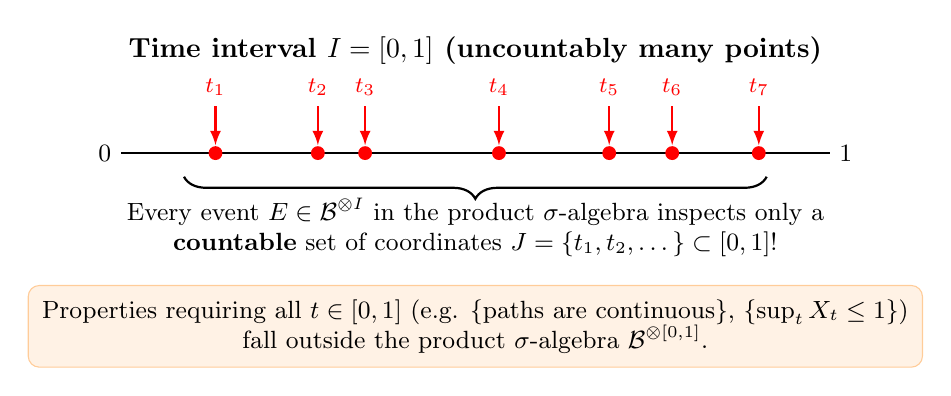
\begin{tikzpicture}[>=latex, font=\small]
  % Time line
  \draw[thick] (0, 0) -- (9, 0);
  \node[left] at (0, 0) {$0$};
  \node[right] at (9, 0) {$1$};
  \node[font=\bfseries] at (4.5, 1.3) {Time interval $I = [0,1]$ (uncountably many points)};

  % Sampled coordinates
  \foreach \x/\lbl in {1.2/t_1, 2.5/t_2, 3.1/t_3, 4.8/t_4, 6.2/t_5, 7.0/t_6, 8.1/t_7} {
    \fill[red] (\x, 0) circle (2.5pt);
    \draw[<-, thick, red] (\x, 0.1) -- (\x, 0.6) node[above, font=\footnotesize] {$\lbl$};
  }

  % Curly bracket
  \draw[thick, decorate, decoration={brace, mirror, amplitude=8pt}] (0.8, -0.3) -- (8.2, -0.3);
  \node[align=center] at (4.5, -0.95)
    {Every event $E \in \mathcal{B}^{\otimes I}$ in the product $\sigma$-algebra inspects only a\\
     \textbf{countable} set of coordinates $J = \{t_1, t_2, \dots\} \subset [0,1]$!};

  \node[align=center, fill=orange!10, draw=orange!40, rounded corners, inner sep=5pt] at (4.5, -2.2)
    {Properties requiring all $t \in [0,1]$ (e.g. $\{\text{paths are continuous}\}$, $\{\sup_{t} X_t \le 1\}$)\\
     fall outside the product $\sigma$-algebra $\mathcal{B}^{\otimes [0,1]}$.};
\end{tikzpicture}
\end{document}
